\documentclass[14pt]{article}
\usepackage{amsmath}
\usepackage{graphicx}
\usepackage{setspace}
\usepackage[utf8]{inputenc}
\usepackage[english]{babel}
\usepackage[backend=bibtex,citestyle=authoryear,url=false,doi=true]{biblatex}
\usepackage[section]{placeins}
\usepackage{fullpage}

\addbibresource{ZoteroBib.bib}

\begin{document}
	
	\title{Literature Review}
	\author{Alec J. Hoyland}
	
	\maketitle
	\doublespacing
	
	\section{Complications Applying Network Theory to Neuroscience}
	
	Twentieth century classical mechanics is sufficient to describe the dynamics of a macroscopic system and the mechanisms which underlie that behavior. This methodology consists of experimental and mathematical analysis and theoretical modeling of physical systems. Analysis permits a physical scientist to make measurements and fit these measurements to mathematical rules, to predict future behavior. In contrast, modeling begins from first principles, establishing and testing a hypothetical set of rules for a system. Good models provide suggestions for experiments which can verify results and provide causal indications between observable, experimental result, and underlying mechanisms.
	
	Similarly, the physics of macroscopic, human-scale systems is sufficiently advanced to permit a physical scientist to readily predict the behavior of a system of arbitrary structure. As above, the caveat here is \textit{given absolute information regarding the initial conditions and rules of evolution}. All models are \textit{wrong} because by necessity reason with incomplete information and make simplifying assumptions. Current theoretical research therefore focuses on systems about which we know comparatively very little: 'the very large, the very small, and the very complex,' (\cite{FeynmanFeynmanLecturesPhysics2013}). Current research at the human-scale is therefore concerned with very complex networks which produce emergent behavior.
	
	Perhaps the most interesting class of networks, from an anthropocentric viewpoint consist of neuronal networks: neurons interacting through synaptic connections. These systems can be describes mathematically as a network, physically as a dynamical system.
	
	The mathematical description of a network begins with a graph, a collection of nodes (vertices) with connections (edges) between them. An edge can be unidirectional (directed) or bidirectional (undirected). In addition, a given edge may have a strength of connection (weight) associated with it. For networks with low-dimensional nodes, behavior of a dynamical system on a network of arbitrary topological complexity can be numerically simulated, though no universal mathematical framework exists for reducing or unfolding these networks (\cite{BarabasiScaleFreeNetworksDecade2009}).
	
	In the case of the nervous system, the smallest discrete nodes are neuronal compartments. These compartments are tacked together to form the morphology of a neuron. An isopotential cell can have one compartment, whereas other models might include 200 or more compartments (\cite{TobinCreationreductionmorphologically2006}). Voltage propagation through compartments within the same neuron is determined by cable theory (\cite{NormanCableTheoryFinite1972}). While information-theoretic methods have been applied to networks in the nervous system (\cite{StemmlerHowvoltagedependentconductances1999}), these networks often contain thousands of nodes abstracted to brain regions, rather than incorporating the biophysical reality of neurons (\cite{PapoComplexnetworktheory2014,ReimannCliquesNeuronsBound2017,BullmoreComplexbrainnetworks2009,BassettNetworkneuroscience2017}). This is due to several problems with applying network theory to realistic neuronal circuits.
	
	First, neuronal networks are structurally complex. A small network with simple oscillatory dynamics, such as linear rate models or analytically-solvable Kuramoto oscillators, can be readily analyzed (\cite{MedvedevSmallworldnetworksKuramoto2014}); however, a real cortical neuron may have up to 10,000 synapses (\cite{DayanTheoreticalNeuroscience2001,AzevedoEqualnumbersneuronal2009}). Second, each node is high-dimensional. Physiologically-realistic models of neuronal activity are high-dimensional nonlinear dynamical systems (\cite{Harris-WarrickDynamicBiologicalNetworks1992,DayanTheoreticalNeuroscience2001}), preventing most graph-theoretic reductions of the network topology. Dynamics in graph theory rely on net flows along edges and processing in vertices. Since the dynamics of a high-dimensional nonlinear oscillator are complex, it is difficult to reduce the dynamics of the network without grossly simplifying the nodes (\cite{ReyesModelingApproachWhy2015,ElicesAsymmetryFactorsShaping2017,DAngeloRealisticmodelingneurons2013}). Third, nearly all computational characteristics of a neuronal network change over time \cite{Harris-WarrickDynamicBiologicalNetworks1992}. Compensation versus environmental perturbations, such as temperature fluctuation, take place over a matter of hours to weeks in invertebrates (\cite{TangPreciseTemperatureCompensation2010,TangRobustnessrhythmiccircuit2012,RoemschiedCellintrinsicmechanismstemperature2014}). Long-term potentiation operates almost immediately and provides a mechanism for longterm associative learning (\cite{NarayananLongTermPotentiationRat2007,Takeuchisynapticplasticitymemory2014}).
	
	Neuronal networks exhibit all of the properties expected of graphs with high-dimensional nodes and yet act on a wide range of timescales. Electrotonus acts in the fast kinetics (\~ 30 ms) of action potentials and the slow kinetics (\~ 1 s) which underly bursting, excitability, and spike propagation. Additionally, the properties which underlie information processing also evolve on ultra-slow (>> 1 s) time-scales of protein turnover, mRNA regulation, and homeostatic control. While detailed investigation of the morphology and excitability of individual neurons has been thoroughly studied, this has not substantially contributed to a comprehensive understanding of large neuronal networks (e.g. the brain) (\cite{KandelPrinciplesneuralscience2013}) because it is poorly understood how neurons in networks of that scale ($10^{10}$ nodes) interact. Fortunately, many networks in neuroscience are organized into motifs which appear again and again in 'small-world' network architecture (\cite{SpornsMotifsBrainNetworks2004}). From studying central pattern generators in great detail, principles governing network motifs can be derived (\cite{MarderCentralpatterngenerators2001a}). For this reason, the examination of high-dimensional small-circuit neuronal networks is crucial to furthering an understanding of the brain.
	
	\section{Neurocomputation}
	The most relevant neurocomputational properties of a neuronal network include the conductances of each neuron, the geometrical structure of the network and the synaptic connections between the neurons.
	
	Neuroscientists have long relied on whole-cell voltage clamp and current clamp recordings, which reveal real-time traces of voltage dynamics of many ion channel types (\cite{HilleIonChannelsExcitable2001}). The excitability of a neuron arises from the combination of ion channels within the cell membrane and the  maximal conductance of a current type is a function of the number of channels (channel density) and the individual efficiency of the channels. Ion flux through transmembrane ion channels produces minute currents which change the electric potential across the membrane (\cite{DayanTheoreticalNeuroscience2001}).
	
	Since the modulation of individual conductances can strongly affect both the passive and active electrical properties of excitable membranes, maintenance of the proper ratio and strength of conductance densities is crucial for effective neuronal activity (\cite{GjorgjievaIntrinsicNeuronalProperties2014,GjorgjievaComputationalimplicationsbiophysical2016}). The excitability and firing properties of a single neuron is a function of its passive electrical properties, intrinsic currents, and inputs and is sensitive to small changes in conductance density (\cite{KaczmarekNeuromodulationBiochemicalControl1987,RinzelFormalClassificationBursting1987,GolowaschCharacterizationstomatogastricganglion1991,GuckenheimerMappingDynamicsBursting1993}). For a network, neuronal properties and synaptic properties must be tuned within characteristic ranges with respect to network output (\cite{MarderCentralpatterngenerators2001a,PrinzComputationalapproachesneuronal2010,DrionIonchanneldegeneracy2015}). Depending on the composition and function of the network, specific properties can be variably important to the degenerate stability of the network activity (\cite{EdelmanDegeneracycomplexitybiological2001,TononiMeasuresdegeneracyredundancy1999}).
	
	The morphological structure and biochemical composition of the cell describes how the signal propagates. Voltage drop over distance can be computed using cable theory (\cite{NormanCableTheoryFinite1972}), in which voltage signals decay through a leaky membrane as a wavefunction. Some neurons rely heavily on morphological tuning to process information (\cite{MainenInfluencedendriticstructure1996,StiefelMappingfunctionneuronal2007,CuntzOnerulegrow2010}).
	
	\section{The Stomatogastric Ganglion (STG)}
	The stomatogastric nervous system (STNS) provides an excellent model system for analyzing how circuit dynamics arise from neuronal properties and network connectivity (\cite{SelverstonCrustaceanStomatogastricSystem1987}). Initial work began in the 1970s (\cite{MaynardSimplernetworks1972}) using the STNS as a model system to understand central pattern generation. Indeed, several properties make this system ideal for electrophysiological and computational analysis.
	
	The STNS consists of a group of four linked ganglia: the paired commissural ganglia (CoG), the  oesophageal ganglion (OG), and the stomatogastric ganglion (STG).  Each of the CoGs contains approximately 400 neurons and the OG contains approximately 18 neurons. The stomatogastric ganglion (STG)  is comprised of approximately 30 neurons – the exact number varies between species and between animals. Most STG neurons fire tonically when pharmacologically isolated but can be induced to burst conditionally under the influence of neuromodulators or graded inhibitory input (\cite{Harris-WarrickDynamicBiologicalNetworks1992}). When the STNS is dissected, it continues to produce fictive motor patterns \textit{in-vitro} which resemble those \textit{in-vivo} (\cite{Harris-WarrickDynamicBiologicalNetworks1992,Nusbaumsmallsystemsapproachmotor2002,SelverstonCrustaceanStomatogastricSystem1987}).
	
	Most synaptic connections in the stomatogastric ganglion (STG) occur between motor neurons, so that the circuit can be isolated from descending interneurons. The fictive motor patterns produced by the STG in-vitro are representative of both the activity of the circuit feedback and the motor output (\cite{MarderPrinciplesrhythmicmotor1996}).
	
	STG neurons have a large soma (typically 50-100 micrometers across) and complex branching morphology. While these cells possess long axons which contribute to descending nerves, much of the arborizations consist of neurites which tangle extensively in the neuropil. This inefficient (\cite{LoebOptimalisngood2012}) wiring follows a space-filling mechanism which results in isopotential membranes (\cite{OtopalikSloppymorphologicaltuning2017}). Therefore, the network relies on intrinsic and synaptic properties instead of morphological tuning to produce target network activity.

	\begin{figure}
		\centering
		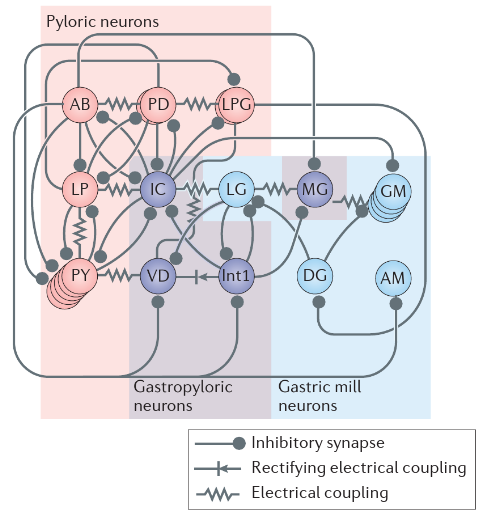
\includegraphics[width=0.5\textheight]{NusbaumMarder2017}
		\caption{Circuit diagram of the stomatogastric nervous system (\cite{NusbaumFunctionalconsequencesneuropeptide2017}).}
	\end{figure}

	STG neurons can be readily examined with electrophysiological methods. It is possible to simultaneously record from 4 intracellular electrodes and 8-12 extracellular nerve electrodes (\cite{MarderPrinciplesrhythmicmotor1996}). Robustness to mechanical insult permits hand-dissection of individual neurons for biochemical characterization and electrophysiological recording for at least 24 hours without incubation (\cite{MarderUnderstandingCircuitDynamics2007,MizrahiLongTermMaintenanceChannel2001}). In addition, intracellular recordings can unambiguously determine cell type between preparations and discriminate between large-amplitude synaptic potentials and subthreshold oscillations (\cite{MarderUnderstandingCircuitDynamics2007,MarderPrinciplesrhythmicmotor1996}).
	
	\section{The Pyloric Rhythm}
	The pyloric rhythm is a triphasic motor pattern almost always continuously expressed in the healthy crustacean (\cite{ClemensLongtermexpressiontwo1998,RezerExpressioncrustaceanpyloric1983}). The frequency and intensity of the rhythmic behavior may vary, but the burst order and duty cycle are maintained in healthy animals (\cite{MarderUnderstandingCircuitDynamics2007}). The canonical pyloric rhythm consists of bursts of action potentials in the pyloric dilator (PD) neurons, followed by bursts in the lateral pyloric (LP) neuron, and finally by bursts in the pyloric (PY) neurons. The inferior cardiac (IC) neuron fires often with the LP neuron and the ventricular dilator (VD) neuron fires frequently with the PY neurons. The anterior burster (AB) interneuron projects through the stomatogastric nerve to the CoGs and is electrically coupled to the twin PD neurons (\cite{Harris-WarrickDynamicBiologicalNetworks1992}).
	
	The cells of the pyloric circuit are synaptically coupled to each other and receive inputs from the anterior CoGs and OG. If glutamatergic inhibitory synapses are blocked with 10 $\mu$M picrotoxin and selective cell-kills by photoinactivation after fluorescent dye injection, the activity of individual cells can be observed (\cite{EisenMechanismsunderlyingpattern1982,JuurlinkNeuralCellSpecification2012}). If descending neuromodulatory inputs are also removed via sucrose block, all cells except for AB fire tonically or quiesce. AB maintains burst characteristics (\cite{SelverstonCrustaceanStomatogastricSystem1987,HooperModulationlobsterpyloric1987,Harris-WarrickDynamicBiologicalNetworks1992}).
	
	In normal pyloric activity, the AB neuron intrinsically oscillates. The PD neurons, electrically coupled to AB, burst in phase. The AB and PD cells inhibit LP and PY, which both burst during PD interphase. LP rebounds from inhibition faster than PY and bursts first. LP and PY are in a 'half-center' oscillator regime of mutual inhibition, so PY neurons rebound and terminate the LP burst.  In this regime, AB is considered the intrinsic pacemaker and AB-PD the pacemaker kernel. The phaselocking of LP and PY during PD interphase is dependent on the intrinsic and synaptic characteristics of the network (\cite{HooperModulationlobsterpyloric1987,HartlinePatterngenerationlobster1979}).
	
	The pyloric rhythm is very robust to perturbation. The circuit is most stable under physiological conditions (11 deg. C with descending neuromodulatory input), however the STG can maintain the phase differences characteristic of pyloric rhythmicity under threefold temperature perturbation and long-term decentralization (\cite{HamoodConsequencesacutelongterm2015,GoldmanGlobalStructureRobustness2001,HaddadCircuitrobustnesstemperature2017}). Since the STG exhibits degenerate morphology which results in isopotential neurons, the circuit stability must be due to intrinsic or synaptic factors.
	
	While the pyloric rhythm is robust to environmental perturbation, it is also susceptible to neuromodulation, allowing for  flexibility in network output while maintaining stability. Neuromodulators are released into the neuropil as a consequence of sensation in the animal or descending modulatory projections from the CoG (\cite{MarderNeuromodulationNeuronalCircuits2012,JohnsonAminemodulationglutamate1997,Nusbaumsmallsystemsapproachmotor2002,MarderCentralpatterngenerators2001a,Nusbaumrolescotransmissionneural2001}).
	
	Unlike many other circuits, the STG is multiply-modulated. The pericardial organ and other neurosecretory organs secrete neuromodulators into the neuropil which colocalize in specific neurons (\cite{Nusbaumrolescotransmissionneural2001,BlitzDifferentProctolinNeurons1999}). In addition, many hormones circulating in the hemolymph can also act as neuromodulators in the STG (\cite{Nusbaumrolescotransmissionneural2001,Harris-WarrickDynamicBiologicalNetworks1992}).
	
	\begin{figure}
		\centering
		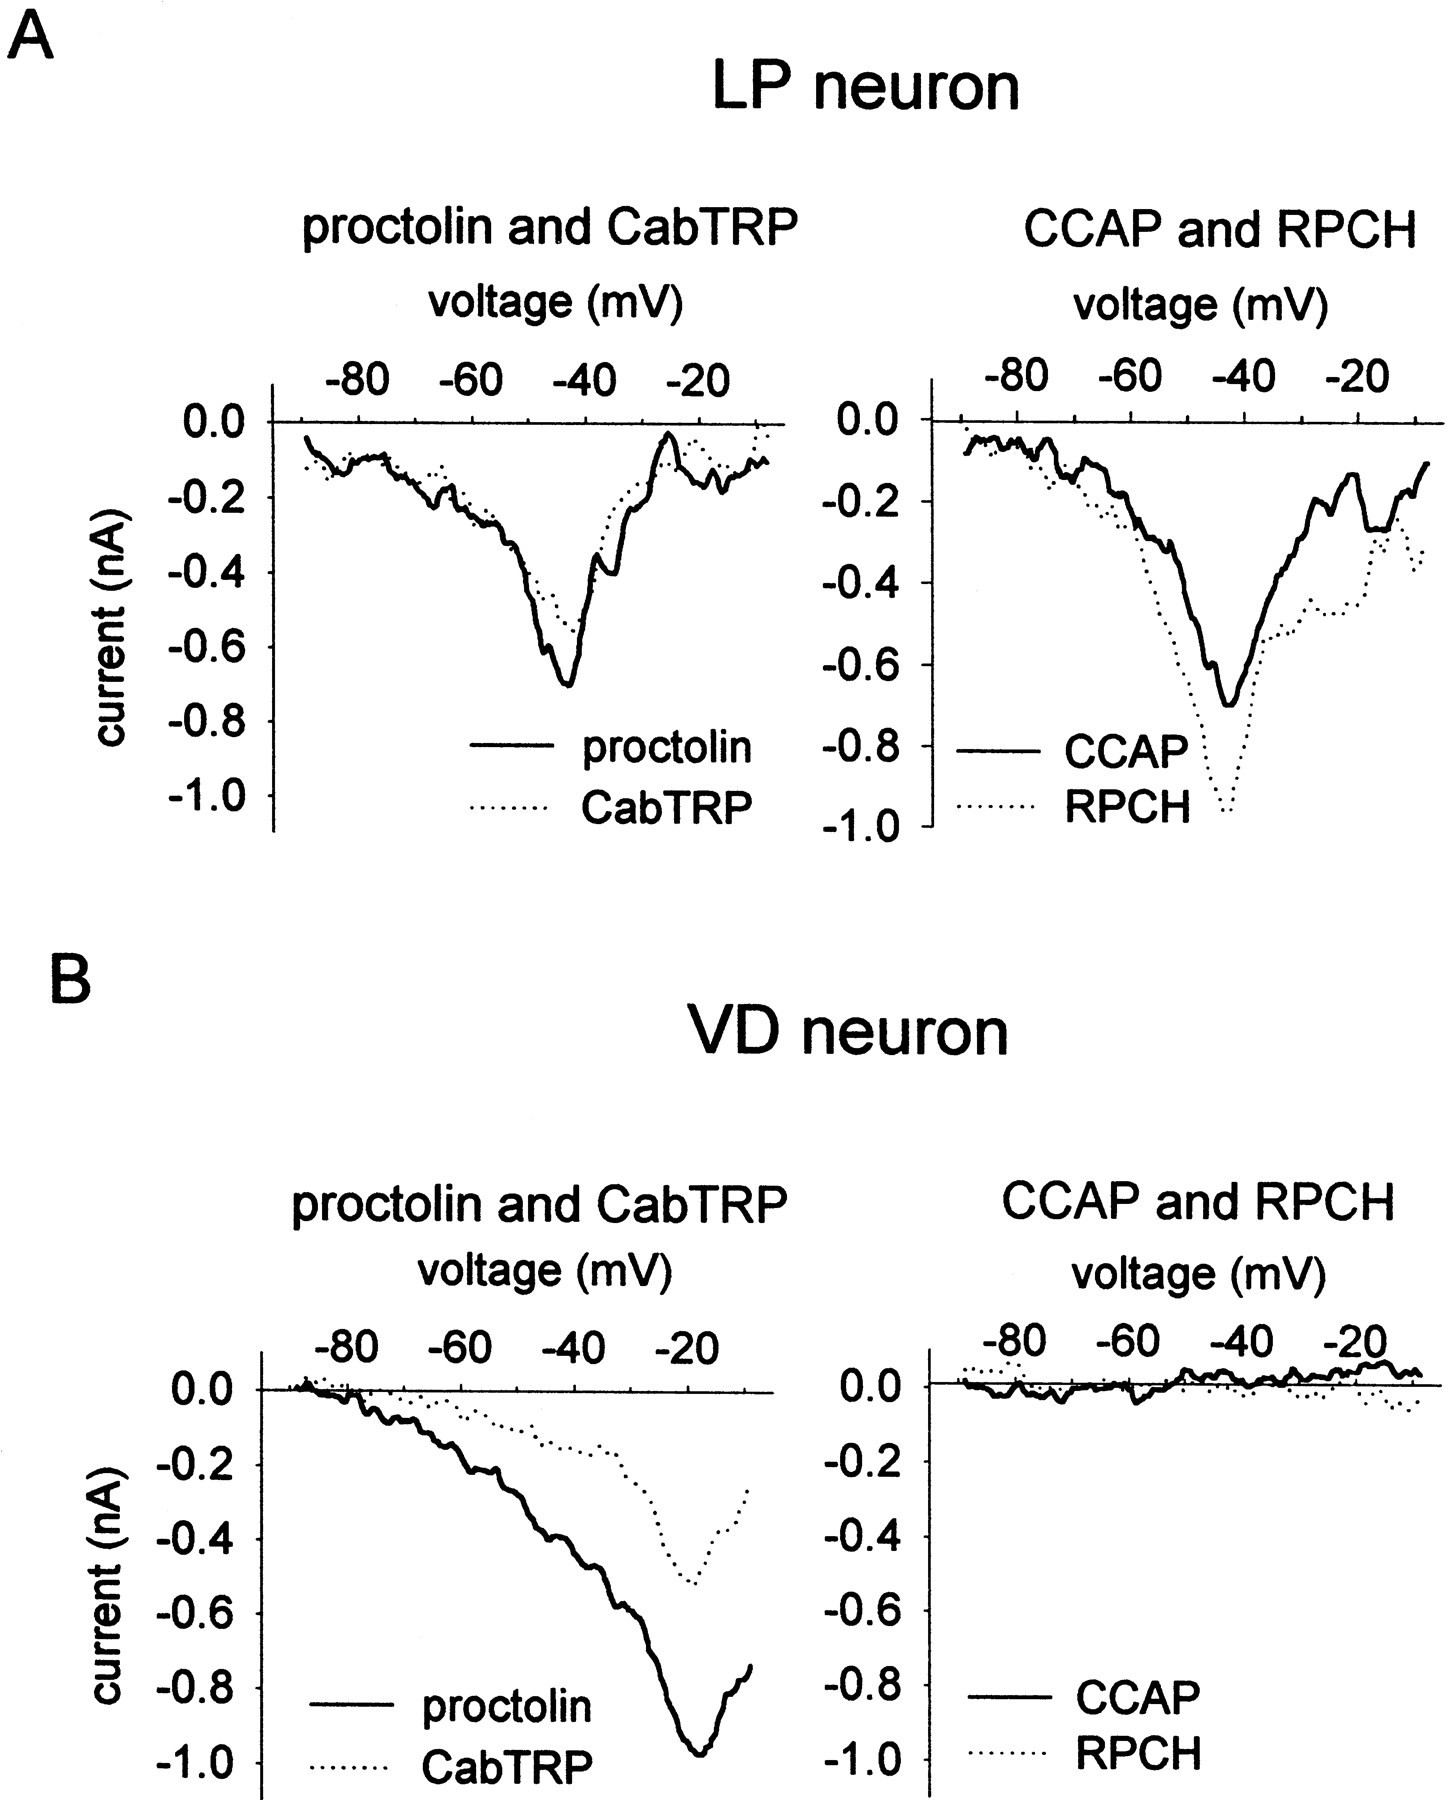
\includegraphics[width=0.5\textheight]{SwensonMarder2001}
		\caption{Current-voltage relation of modulatory input current in STG cells (\cite{SwensenModulatorsconvergentcellular2001}).}
	\end{figure}

	In general, neuromodulators enhance the flexibility of neuronal networks. In one such method, neuromodulators activate a new current (\cite{GolowaschIoniccurrentslateral1992,GolowaschProctolinactivatesinward1992}). In my proposed thesis, the perturbation considered will be neuromodulation, specifically, the activation of $I_{MI}$, an excitatory modulatory input current. 
	
	All cells of the pyloric network are capable of activating $I_{MI}$ through modulatory action though they vary in its response. Differential receptor expression leads to variability and flexibility in cellular and network response to modulatory chemicals. The effects of neuromodulators can be mimicked \textit{in-vitro} using dynamic clamp to inject current commensurate to a predetermined current-voltage relation (\cite{SharpDynamicclampcomputergenerated1993,SwensenModulatorsconvergentcellular2001,SwensenMultiplepeptidesconverge2000}).
	
	\section{Modeling the Stomatogastric Ganglion (STG)}
	In 1995, Turrigiano et al. identified nine voltage- and time-dependent conductances to simulate conductance-based STG neurons using the Hodgkin-Huxley formalism (\cite{Hodgkincomponentsmembraneconductance1952,HodgkinMeasurementcurrentvoltagerelations1952,Hodgkinquantitativedescriptionmembrane1952,FosterSignificanceconductancesHodgkinHuxley1993,TurrigianoSelectiveregulationcurrent1995}). Ionic gating variable curves were fit to IV-curve voltage-clamp data. Other experiments used dynamic clamp to test model currents in real neurons (\cite{SharpDynamicclampcomputergenerated1993,DestexheDynamicClampPrinciplesApplications2009}). While other conductance-based models in the STG had been developed prior (\cite{LeMassonActivityDependentRegulationConductances1993,AbbottAnalysisNeuronModels1993}), Turrigiano \textit{et al.} has been cited frequently in more recent STG models because of its involved description of current dynamics in STG models (\cite{Liumodelneuronactivitydependent1998,PrinzAlternativehandtuningconductancebased2003,PrinzSimilarnetworkactivity2004,PrinzComputationalapproachesneuronal2010,SoofiPhasemaintenancerhythmic2014}). The complete description of major conductances in STG neurons has been built upon, rather than reinvented.
	
	Strogatz explains that, “No insight is gained if the model is as perplexing as the phenomena it is supposed to describe” (\cite{StrogatzSyncEmergingScience2003}). To this end, conductance-based models of the STG have strived for verisimilitude only so much as to encompass the burst characteristics, phase relationships, and other neurocomputational properties of the circuit, rather than to mimic the precise waveforms of intracellular recordings. Robustness to modulation remains a key feature of the pyloric rhythm.
	
	A single-compartment conductance-based model database demonstrated that diverse sets of maximal conductances can produce spiking activity. Neurons can be approximated as isopotential due to morphological degeneracy (\cite{OtopalikSloppymorphologicaltuning2017}). While the set of points in conductance space which elicit spiking behavior is not ergodic, the spiking subspace is much larger than initially expected (\cite{PrinzAlternativehandtuningconductancebased2003,GoldmanGlobalStructureRobustness2001,GolowaschFailureaveragingconstruction2002}). In three-cell networks (ABPD composite, LP, PY), simulations elicited similar network activity from disparate network parameters, showing the theoretical possibility of significant network degeneracy. The intrinsic maximal conductances were selected from the STG model database (\cite{PrinzAlternativehandtuningconductancebased2003}), which in turn were based upon the original recordings in \cite{TurrigianoSelectiveregulationcurrent1995}. These theoretical intuitions were supported by mRNA assays, demonstrating significant animal-to-animal variability in maximal conductances (\cite{SchulzVariablechannelexpression2006,GoaillardFunctionalconsequencesanimaltoanimal2009,BucherAnimaltoanimalvariabilitymotor2005,HamoodAnimaltoanimalvariabilityneuromodulation2014}).
	
	Models of network activity in the STG have demonstrates degeneracy (\cite{PrinzSimilarnetworkactivity2004}) and pacemaker models have shown robustness to environmental perturbation (\cite{CaplanManyParameterSets2014}).
	
	Degeneracy can be thought of as a form of redundancy, in which the functions or capabilities of a biological system overlap in order to compensate for a perturbation or failure within the system at-large  (\cite{EdelmanDegeneracycomplexitybiological2001,WhitacreDegeneracydesignprinciple2010}).
	
	While each subfield in biology prefers its own metric for robustness (\cite{StellingRobustnessCellularFunctions2004}), robustness is generally understood to be the insensitivity of some functional system to a set of distinct conditions. For example, triphasic rhythmicity is necessary for innervation of pyloric muscles in crustaceans, so the ability to maintain phase under increasing temperature is a form of robustness (\cite{SoofiPhasemaintenancerhythmic2014}). In this way, robustness is considered inextricably linked to biological fitness (\cite{KitanoBiologicalrobustness2004}). If the pyloric rhythm malfunctions significantly, the crab would not be able to digest, as the pylorus opens from the stomach into the lower digestive tract. In a more stark example, the central patterns governing respiration in mammals must be highly robust, as cessation results in death of the organism (\cite{BellinghamDrivingrespirationrespiratory1998}).
	
	\section{Conductance-Based Models}
	The Hodgkin-Huxley formalism envisions excitable membranes as capacitors with parallel variable resistors (intrinsic conductances) which act to change the membrane potential (Hodgkin and Huxley 1952). The membrane voltage evolves over time as a function of the sum of the currents. This is described by the conservation of current equation:
	
	\[C_m \frac{dV_m}{dt} = - \sum_{i} I_i = - \sum_{i} \bar{g}_{i} {m_i}^{p_i} {h_i}^{q_i} (V_m - E_i) \]
	
	The $i^{th}$ current is of the form:
	
	\[I_i = \bar{g}_{i} {m_i}^{p_i} {h_i}^{q_i} (V_m - E_i)\]
	
	This form follows from Ohm’s Law for a variable resistor. The electrochemical potential $V_m - E_i$ consists of the membrane potential $V_m$ and the reversal (Nernst) potential $E_i$ of the ion species across the membrane. The conductance is defined as the inverse of the resistance $g(V) = \bar{g} m^p h^q$ in which $\bar{g}$ represents the maximal conductance density. The ionic gating variables $m$ and $h$ with their integer exponents $p$ and $q$ represent proportions of channels open or inactivated.
	
	In most models, the reversal potentials $E_i$ and the specific membrane capacitance $C_m$ are treated as constant. In the first case, this is because high concentrations of sodium and potassium ions and chloride counter-ions are not strongly affected by the minute ion flux resulting in intrinsic currents. The logarithmic ratio of concentrations inside and outside must change significantly for this physical phenomenon to be worth including in the model. Since there is such a small intracellular concentration of calcium ions, intracellular calcium concentration is typically modeled as an additional parameter (\cite{Liumodelneuronactivitydependent1998}8). Work by Huxley shows that the specific membrane capacitance varies on $[9,15] ~nF/mm^2$, so it is traditional to set $C_m =  1 nF/mm^2$ (\cite{Hodgkinquantitativedescriptionmembrane1952,HilleIonChannelsExcitable2001}).
	
	Intracellular calcium concentration changes as a function of calcium buffering rate and calcium currents. The primary form of this equation is simple:
	
	\[\tau_{Ca} \frac{d[Ca^{2+}]}{dt} = [Ca^{2+}]_{\infty} - [Ca^{2+}] \]
	
	The steady-state function $[Ca^{2+}]_{\infty}(I_{Ca})$ is a function of calcium currents; the actual calcium concentration  lags with the time constant.
	
	\[[Ca^{2+}]_{\infty}(I_{Ca}) = -f \sum_{Ca} + [Ca^{2+}]_{0} \]
	
	In this context, $f$ is a buffering coefficient. It translates the calcium flux (in units of current per area) into a steady-state concentration. $[Ca^{2+}]_0$ represents the equilibrium intracellular calcium concentration.
	
	Similarly, each ionic gating function is of the form:
	
	\[\tau_{z} \frac{dz}{dt} = z_{\infty} - z \]
	
	where $z(V,t) \rightarrow (m,h)$. The steady states $z_\infty$ generally take the form of Boltzmann functions which were fit from experiment (\cite{TurrigianoSelectiveregulationcurrent1995}). The membrane potential at which a conductance is half open (e.g. $m=0.5$) is called the half-potential.  From the complex nonlinear interplay of several conductances, neuronal behavior emerges.
	
	\section{Novel Computational Implementation}
	In collaboration with Srinivas Gorur-Shandilya, I have developed a simulation toolbox for conductance-based models. The core code is written in $\texttt{C++}$ and transpiled and compiled from $\texttt{MATLAB}$ (The Mathworks) using the $\texttt{MEX}$ compiler.
	
	Models were simulated in \texttt{MATLAB} with a time resolution of 50 microseconds for 10 seconds. Speed is reported in ratios of real-time performance (e.g. 10x means 10 seconds of simulation-time was completed in 1 second of real-time).
	
	Custom software packages \texttt{procrustes} implements a pattern search algorithm in \texttt{MATLAB} to optimize tunable network parameters. In addition \texttt{psychopomp} recruits nodes to simulate in parallel.
	
	\section{Robustness in STG Pacemaker Models}
	Previous research by Astrid Prinz (\cite{PrinzAlternativehandtuningconductancebased2003,PrinzSimilarnetworkactivity2004}) demonstrated the effectiveness of single-compartment models in exploring network degeneracy. In order to examine the effects of robustness, excitatory modulatory input current $I_{MI}$ was applied to cells from the Prinz database (\cite{PrinzAlternativehandtuningconductancebased2003}). The dynamics for this current were taken from previous pacemaker models (\cite{CaplanManyParameterSets2014}).
	
	The current is $I_{MI} = \bar{g}_{MI} m_{MI} (V_m - E_i)$ where $E_{MI} = 0~mV$ and $m^{MI}_\infty(V) = \frac{1}{1 + exp(\frac{V + 38}{3.05})}$ and $\tau_{MI} = 0.5~ms$. Physiological ranges for maximal conductances are $\bar{g}_{MI} \in [0,10]~\mu S/mm^2$.
	\begin{figure}
		\centering
		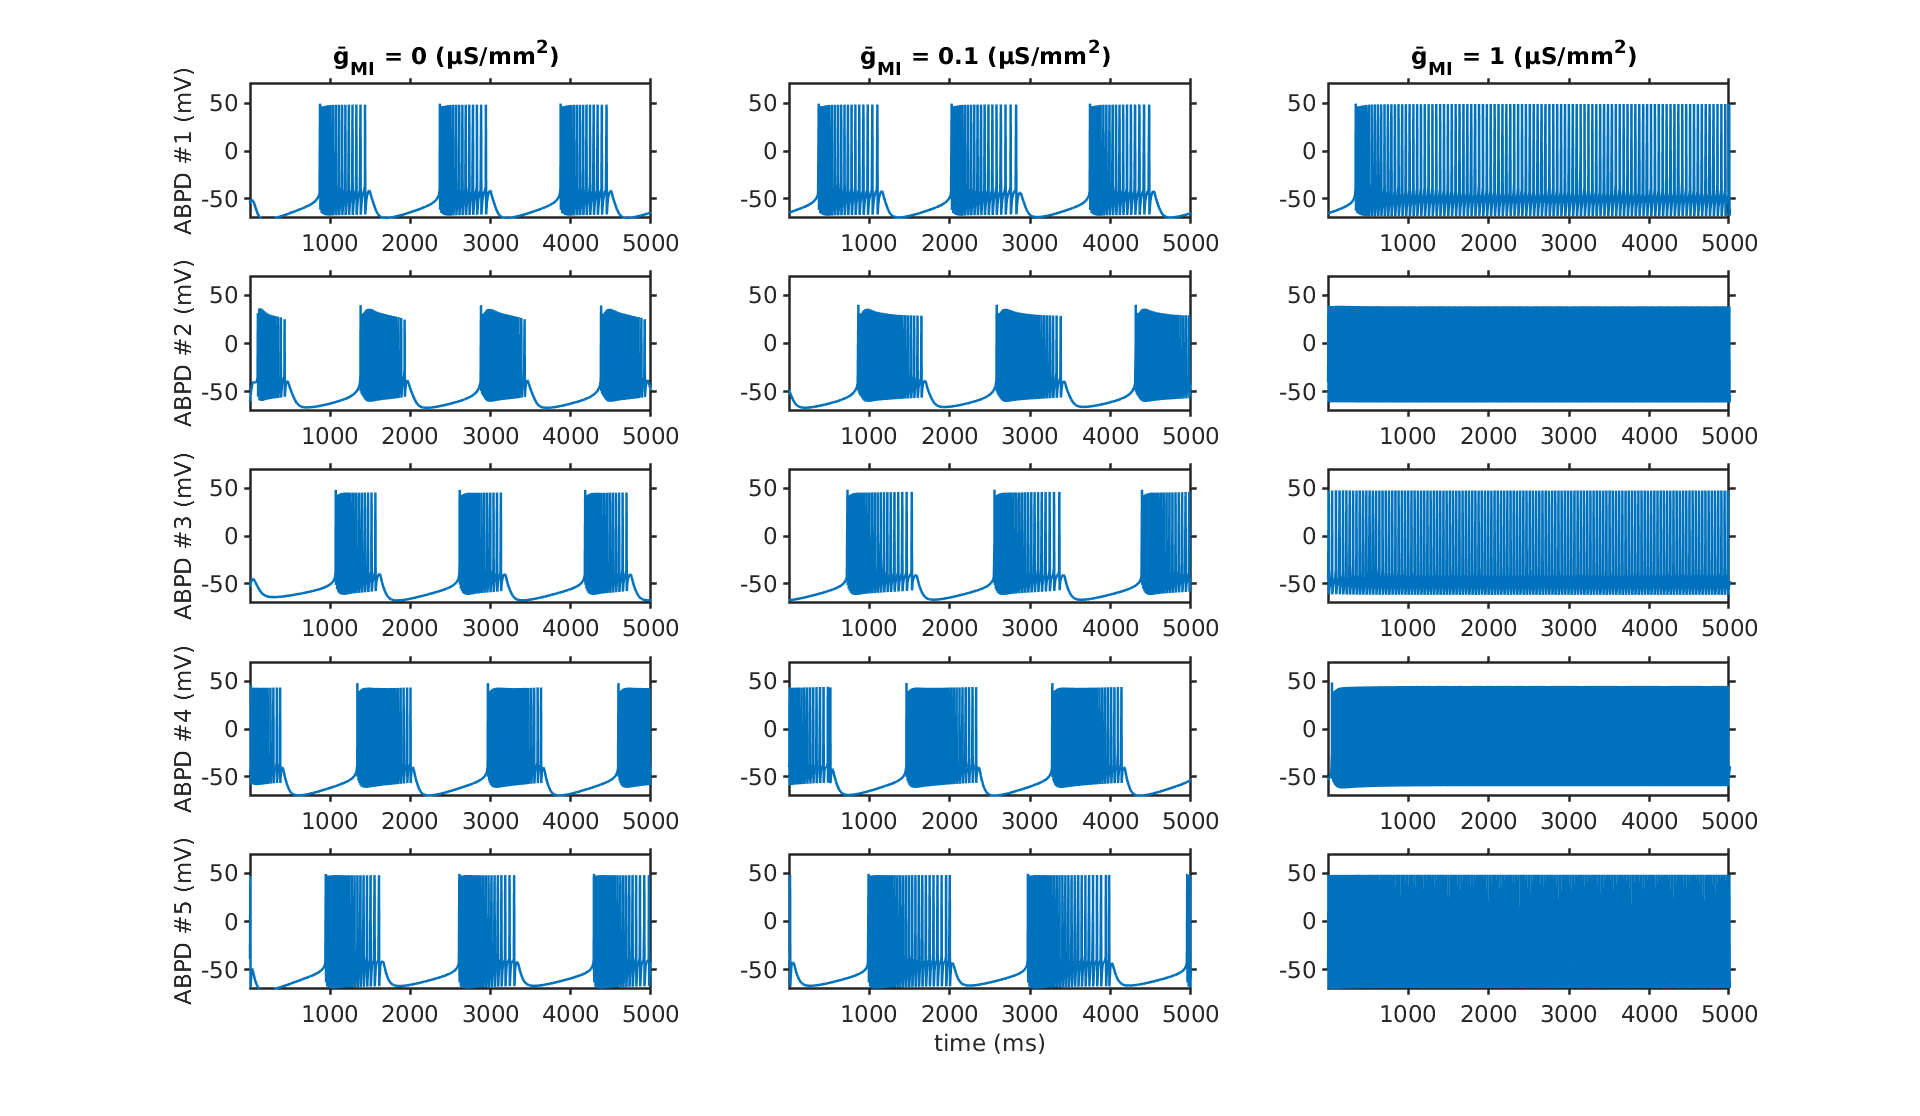
\includegraphics[width=0.8\textheight]{PrinzABPDwithMI}
		\caption{Prinz ABPD pacemaker models were simulated with $I_{MI}$ at three maximal conductances, demonstrating that the models are not robust.}
	\end{figure}
	While the bursting models of PD activity may function well in demonstrations of network degeneracy, application of modulatory input perturbation to the system results in complete breakdown of network behavior.
	
	\section{Thesis}
	The neurons that generate the pyloric rhythm of the STG display both spike-mediated and graded release of transmitter (\cite{ThirumalaiRedPigmentConcentrating2006,RaperNonimpulsemediatedsynaptictransmission1979}). The phase relationships in the pyloric rhythm depend on the intrinsic currents of each neuron in the circuit and the strength and dynamics of the synaptic connections (\cite{EisenMechanismsunderlyingpattern1982,Harris-WarrickDynamicBiologicalNetworks1992,HartlinePatterngenerationlobster1979,MarderUnderstandingCircuitDynamics2007}). Consequently, neuromodulators which alter these properties in the network can alter the phase of the neurons in the motor output.
	
	By blocking sodium channels with tetrodotoxin (TTX), it is possible to assess the extent to which graded transmission can account for the generation of the pyloric rhythm under neuromodulation (Rosenbaum \& Marder, unpublished).
	\begin{figure}
		\centering
		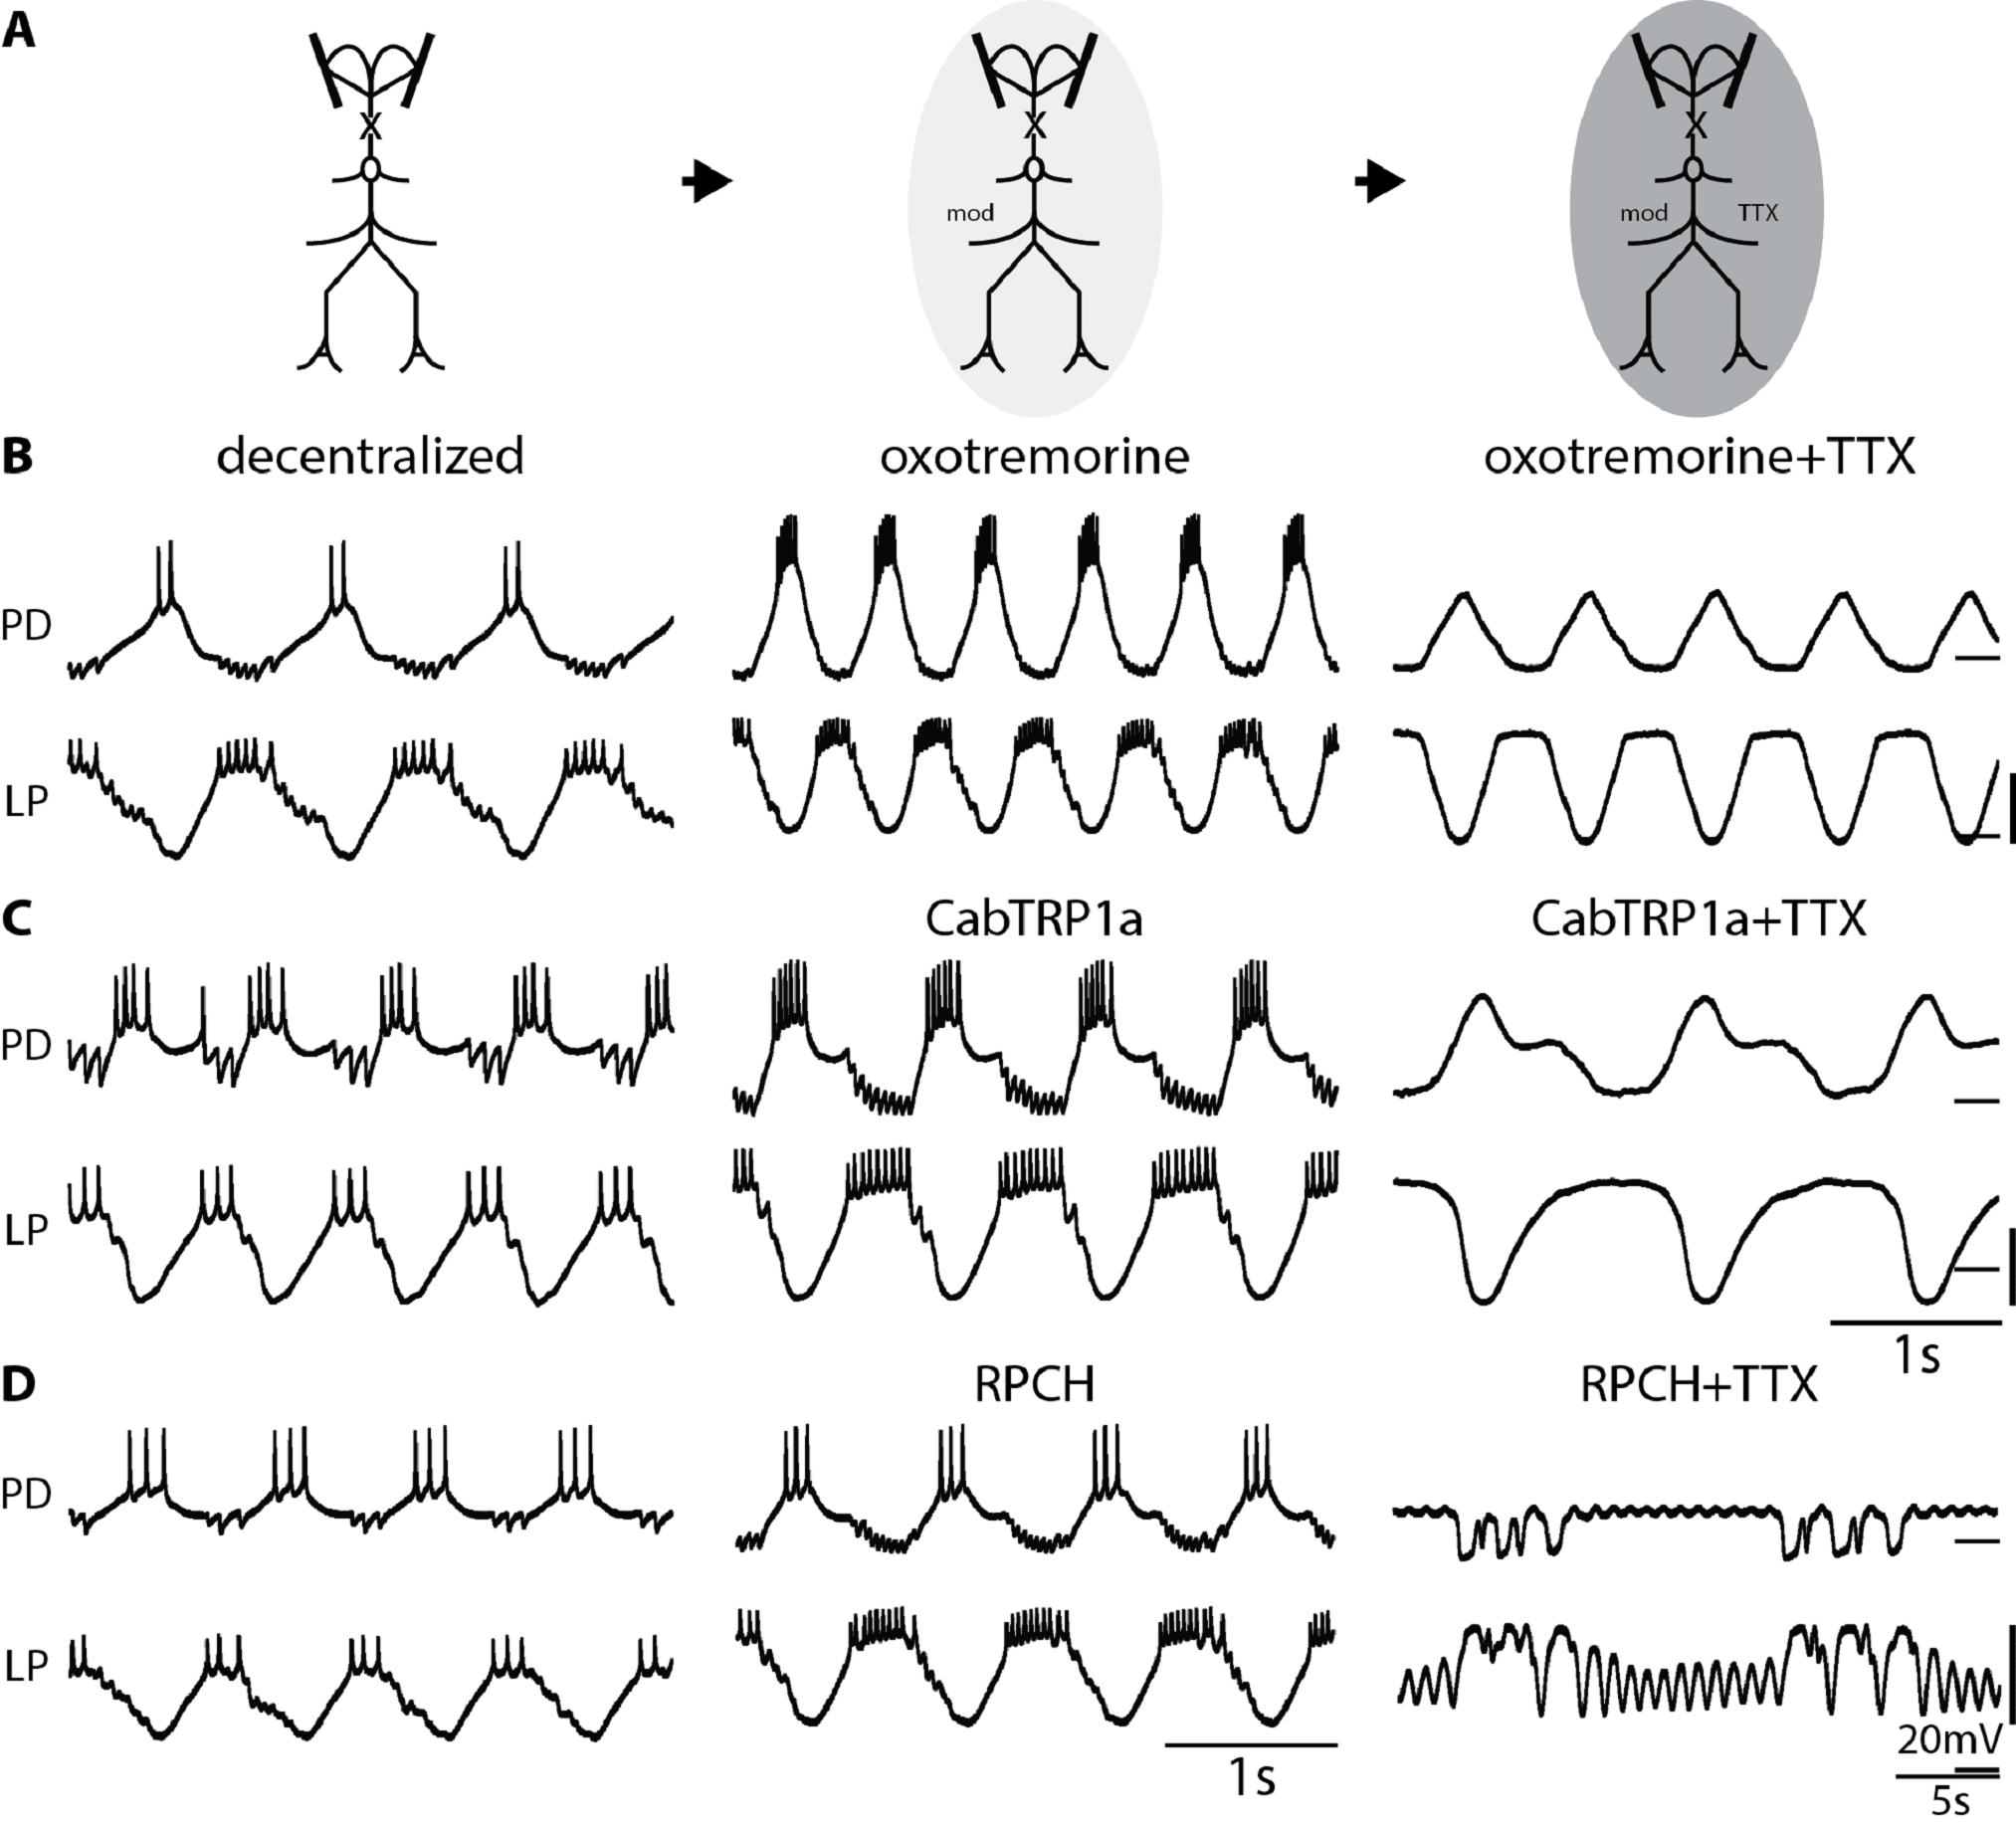
\includegraphics[width=0.5\textheight]{Rosenbaum2017Fig2}
		\caption{Effects of modulators and modulators in TTX on the pyloric rhythm. \textbf{A}, Schematic of the STNS during different experimental conditions (from left to right): decentralized, modulator application, modulator and TTX application. \textbf{B-D}, Intracellular recordings of the pyloric dilator neuron (PD) and lateral pyloric neuron (LP) in the three different conditions. In the decentralized preparation the frequency decreased, phase relationships remain similar (all left panels). \textbf{B}, Application of the muscarinic agonist oxotremorine strongly activates the pyloric rhythm and increases burst frequency. Co-application of oxotremorine and TTX abolishes spiking but leaves the slow wave oscillations almost unchanged. \textbf{C}, CabTRP1a produces a strong pyloric rhythm, after addition of TTX slow wave remains but rhythm slows down. \textbf{D}, RPCH produces a robust pyloric rhythm, after the addition of TTX oscillations with two time components emerge. Vertical scale bars correspond to 20mV in all subplots. Dashed lines at -50mV. (Rosenbaum \& Marder, unpublished).}
	\end{figure}

	A first parameter search (using \texttt{procrustes}) will identify AB-like neuronal models which maintain PD phase and burst-frequency when perturbed by modulatory input into AB. These models will be combined with LP and PY models from the Prinz database. A second parameter search will identify synaptic conductances which produce triphasic rhythmic activity for the cohort of AB, PD, LP, and PY models. The algorithm will select for network parameters which increase burst-frequency over increasing modulation into AB while maintaining phase relationships. 
	
	Finally, the set of networks passing all tests will be subjected to simulated TTX $(\bar{g}_{NaV} = 0)$ in order to replicate and understand unpublished data by P. Rosenbaum.

	\medskip
	\FloatBarrier
	\printbibliography

\end{document}
